%% DOCUMENTCLASS %%
\documentclass[12pt, a4paper]{article}
% \documentclass{scrartcl}

%%%% PACKAGES %%%%

%% RANDOM %%
\usepackage[usenames, dvipnames, svgnames, x11names, table]{xcolor}
\usepackage[nohyperref]{doc}
\usepackage{background}

%% FONTS %%
\usepackage[T1]{fontenc}
\usepackage[normalem]{ulem}



%% IMAGES %%
\usepackage{graphicx}
\usepackage{float}
\usepackage{subcaption}

%% GRAPHICS %%
\usepackage{tikz}
\usepackage{pgfplots,pgf-pie}
\pgfplotsset{compat=1.18}

%% MATH %%
\usepackage{amsmath}
\usepackage{amsfonts}
\usepackage{amssymb}
% \usepackage{amsthm} out of scope

% PHYSICS %%
\usepackage{physics}

%% TABLE and LIST %%
\usepackage{multirow}
\usepackage[shortlabels]{enumitem}

%% GEOMETRY %%
% \usepackage{geometry}
% \geometry{margin=1in, a4paper}

%% REFERENCES %%
\usepackage[style=ieee, sorting=nyt]{biblatex}
\addbibresource{references.bib}

%% HYPERREF %%
\usepackage{hyperref}
\hypersetup{
    draft = false,
    linktocpage = true,
    colorlinks=true,
    linkcolor=DeepSkyBlue4,
    filecolor=magenta,      
    urlcolor=DeepPink,
    citecolor=Green4,
    pdftitle={LaTeX Handout Slashdot},
    pdfauthor={Piyush, Sabarno, Debayan, Gautam},
    pdfsubject={Slashdot},
    pdfkeywords={handout, latex, slashdot},
    pdfpagemode=FullScreen,
}

%% TITLE PAGE %%
\title{\Huge \LaTeX{} Workshop Handout}
% \author{Piyush Kumar Singh\footnote{22MS027} \\ Debayan Sarkar\footnote{22MS002} \\ Sabarno Saha\footnote{22MS037} \\ Gautam Singh\footnote{22MS023}}

\author{\large
    Debayan Sarkar
        \thanks{{\href{https://thesillycoder.github.io}{TheSillyCoder.github.io}}}
        \\\href{mailto:ds22ms002@iiserkol.ac.in}{22MS002} \and
    Gautam Singh
        % \thanks{{}}
        \\\href{mailto:gs22ms023@iiserkol.ac.in}{22MS023} \and
    Piyush Kumar Singh
        \thanks{{\href{https://iampiyushkrsingh.github.io}{iamPiyushKrSingh.github.io}}}
        \\\href{mailto:pks22ms027@iiserkol.ac.in}{22MS027} \and
    Sabarno Saha
        % \thanks{{}}
        \\\href{mailto:ss22ms037@iiserkol.ac.in}{22MS037}
}

\date{
    \normalsize
    \textit{Indian Institute of Science Education and Research, Kolkata, \\
        Mohanpur, West Bengal, 741246, India.}
}

%% DOCUMENT STARTS %%
\begin{document}
\large

\begin{titlepage}
% Remove the watermark
\backgroundsetup{contents={}, scale=0.5, opacity=0.05}

\begin{figure}
\centering

\includegraphics[width = \textwidth]{banner-w.png}
\end{figure}

\vspace{10ex}

\maketitle

\end{titlepage}

\backgroundsetup{contents=
\includegraphics{banner-w.png}, scale=0.35, opacity=0.05}
\tableofcontents
\pagebreak
\section{What is \textrm{\LaTeX}?}

\LaTeX{} is a software system for high-quality typesetting. It's commonly used for academic papers, scientific reports, books, and other documents that require precise formatting and complex layouts. It is based on the \TeX\ typesetting system created by Donald Knuth. Unlike word processors like LibreOffice Writer, whose philosophy is based on "WYSIWYG", \LaTeX\ focuses on the content of your document and then automatically takes care of the formatting based on a set of instructions you provide. This can be more time-consuming to learn initially, but it can save you time and frustration in the long run, especially for long and complex documents.

Here are some key features of \LaTeX:
\begin{itemize}
    \item {Document Classes}%: \LaTeX\ supports various document classes, such as \texttt{article}, \texttt{report}, and \texttt{book}, each designed for specific types of documents. These classes define the overall layout and formatting of the document.

    \item {Packages}%: \LaTeX\ allows users to include additional functionality and formatting options through packages. Users can import packages to extend the capabilities of \LaTeX\ and customize the appearance of their documents.

    \item {Mathematics and Equations}%: \LaTeX\ is viral in academia and scientific writing due to its robust support for mathematical symbols and equations. It provides an efficient and consistent way to typeset complex mathematical formulas.

    \item {Cross-Referencing}%: \LaTeX\ simplifies the process of cross-referencing within a document. Users can easily refer to sections, figures, tables, and equations using labels and references.

    \item {Bibliography Management}%: \LaTeX\ integrates with \BibTeX, a program that helps manage bibliographies and citations. This is especially useful for academic and research papers.

    \item {Professional Typesetting}%: \LaTeX\ produces high-quality, professional-looking documents with precise fonts, spacing, and layout control. It is widely used in creating academic papers, theses, books, and technical documents.
\end{itemize}

\section{Structure of \texttt{.tex} file}

This section will discuss the following part of a generic \texttt{.tex} file.

\subsection{Document Class}

In a typical \verb|.tex| file, the first line declares documentclass. 

\begin{verbatim}
\documentclass[12pt,  a4paper, two columns]{article}
\end{verbatim}

\subsection{Preamble}

The preamble in a \LaTeX\ document is the section between the \verb|\documentclass| declaration and the \verb|\begin{document}| command. It plays a crucial role in setting up the document's overall formatting, style, and additional features.\\[1.2ex]
In this section, we do the following things:
\begin{enumerate}
\item Package Inclusion
\item Title, Author and Date

For this document we have defined the variable in preamble as follows:
\begin{verbatim}
\title{\Huge \LaTeX{} Workshop Handout}

\author{\large
Debayan Sarkar
\thanks{{\href{https://thesillycoder.github.io}{TheSillyCoder.github.io}}}
\\\href{mailto:ds22ms002@iiserkol.ac.in}{22MS002} \and
Gautam Singh
\\\href{mailto:gs22ms023@iiserkol.ac.in}{22MS023} \and
Piyush Kumar Singh
\thanks{{\href{https://iampiyushkrsingh.github.io}{iamPiyushKrSingh.github.io}}}
\\\href{mailto:pks22ms027@iiserkol.ac.in}{22MS027} \and
Sabarno Saha
\\\href{mailto:ss22ms037@iiserkol.ac.in}{22MS037}
}

\date{
\normalsize
\textit{Indian Institute of Science Education and Research, Kolkata, \\
Mohanpur, West Bengal, 741246, India.}
}
\end{verbatim}

And for the title page we used the following way:
\begin{verbatim}
\begin{titlepage}
\% Remove the watermark
\backgroundsetup{contents={}, scale=0.5, opacity=0.05}

\begin{figure}
\centering

\includegraphics[width = \textwidth]{banner-w.png}
\end{figure}

\vspace{10ex}

\maketitle

\end{titlepage}
\end{verbatim}


\item Custom Commands and Settings
\item Bibliography Setup (if using BibLaTeX)
\end{enumerate}

\subsection{Main Body}

The main body of a \LaTeX\ document is the enclosed portion between \verb|\begin{document}| and \verb|\end{document}| command. It is where you write the actual content of your document, such as text, sections, mathematical equations, figures, and tables.

\section{Document Sectioning}

The document sectioning can be done up to 7 levels:
\begin{itemize}
    \item Part : \verb|\part|
    \item Chapter : \verb|\chapter|
    \item Section : \verb|\section|
    \item Sub-Section : \verb|\subsection|
    \item Sub-Sub-Section : \verb|\subsubsection|
    \item Paragraph : \verb|\paragraph|
    \item Sub-Paragraph : \verb|\subparagraph|
\end{itemize}

Note: To use part and chapter commands, you must use \verb|report| or \verb|book| documentclass.

You can force a line break by using \verb|\\|. Use \verb|\pagebreak| to force a page break.

\section{Font Style, Size and Color}

\subsection{Font Style}

We can stylize the fonts used in our document by following commands:
\begin{itemize}
    \item \textbf{Bold Face}:
    \begin{verbatim}
This is \textbf{bold text}.
    \end{verbatim}

    \item \textit{Italics}:
    \begin{verbatim}
This is \textit{italic text}.
    \end{verbatim}
image
    \item \uline{Underline}:
    \begin{verbatim}
\usepackge[normalem]{ulem} % put in preamble

---

This is \uline{underlined text}.
    \end{verbatim}

    \item \emph{Emphasis}: It is a very context-dependent command but is very useful when we want to emphasize a part of text (without worrying about the formatting)
\end{itemize}

\subsection{Font Size}

We have an extensive range of font sizes in \LaTeX{}.
\begin{itemize}[$\odot$]
    \item \verb|\tiny{Tiny Size}| : {\tiny Tiny Size}
    \item \verb|\scriptsize{Script Size}| : {\scriptsize Script Size}
    \item \verb|\footnotesize{Footnote Size}| : {\footnotesize Footnote Size}
    \item \verb|\small{Small Size}| : {\small Small Size}
    \item \verb|\normalsize{Normal Size}| : {\normalsize Normal Size}
    \item \verb|\large{large Size}| : {\large large Size}
    \item \verb|\Large{Large Size}| : {\Large Large Size}
    \item \verb|\LARGE{LARGE Size}| : {\LARGE LARGE Size}
    \item \verb|\huge{huge Size}| : {\huge huge Size}
    \item \verb|\Huge{Huge Size}| : {\Huge Huge Size}
\end{itemize}

\subsection{Font Color}

Use the \textcolor{MidnightBlue}{\texttt{xcolor}} package to set the text colour. Include \verb|\usepackage{xcolor}| in the preamble.

\begin{verbatim}
\usepackage{xcolor} % put this in preamble


---

\textcolor{red}{This is red text.}
\end{verbatim}
\textcolor{red}{This is red text.}

\section{Math}
While writing math in \LaTeX{}, there are two environments via which math can be displayed, namely Inline math and Display math
\begin{itemize}
    \item[\textbf{Inline Math}] Inline math is the environment used when Math is displayed inside a paragraph. The syntax for inline math is \verb|$ ... $ or \( ... \)|.
    \item[\textbf{Display Math}] Display Math is the environment used when math is displayed not in a paragraph but on its own. The syntax for display math is multiple 
    \verb|$$ ... $$ or \[ ... \]|. 
\end{itemize}
Here is an example of display versus inline math. So \((a+b)^2 = a^2+2ab+b^2\) is inline math whereas 
\[(a+b)^2 = a^2+2ab+b^2\] is display math.
\subsection{Important Functions}
Listed here are some important functions:
\begin{itemize}
    \item \verb|\frac{355}{113}| $ \rightarrow \frac{355}{113}$ 
    \item \verb|\int_{0}^{\infty}dx| $ \rightarrow \int_{0}^{\infty}dx$
    \item \verb|\int\limits^{0}_{\infty}dx|$ \rightarrow \int\limits_{0}^{\infty}dx$
    \item \verb|\iiint dv| $\rightarrow \iiint dv$
    \item \verb|\oint dr| $\rightarrow \oint dr$
    \item \verb|\sum_{n=1}^{\infty}| $\rightarrow \sum_{n=1}^{\infty}$
    \item \verb|\sum\limits_{n=1}^{\infty}| $\rightarrow \sum\limits_{n=1}^{\infty}$
    \item \verb|\prod\limits_{n=1}^{\infty}| $\rightarrow \prod\limits_{n=1}^{\infty}$

\end{itemize}

\subsection{Greek Symbols}
Here is a ready reference for Greek symbols: 
\begin{center}
        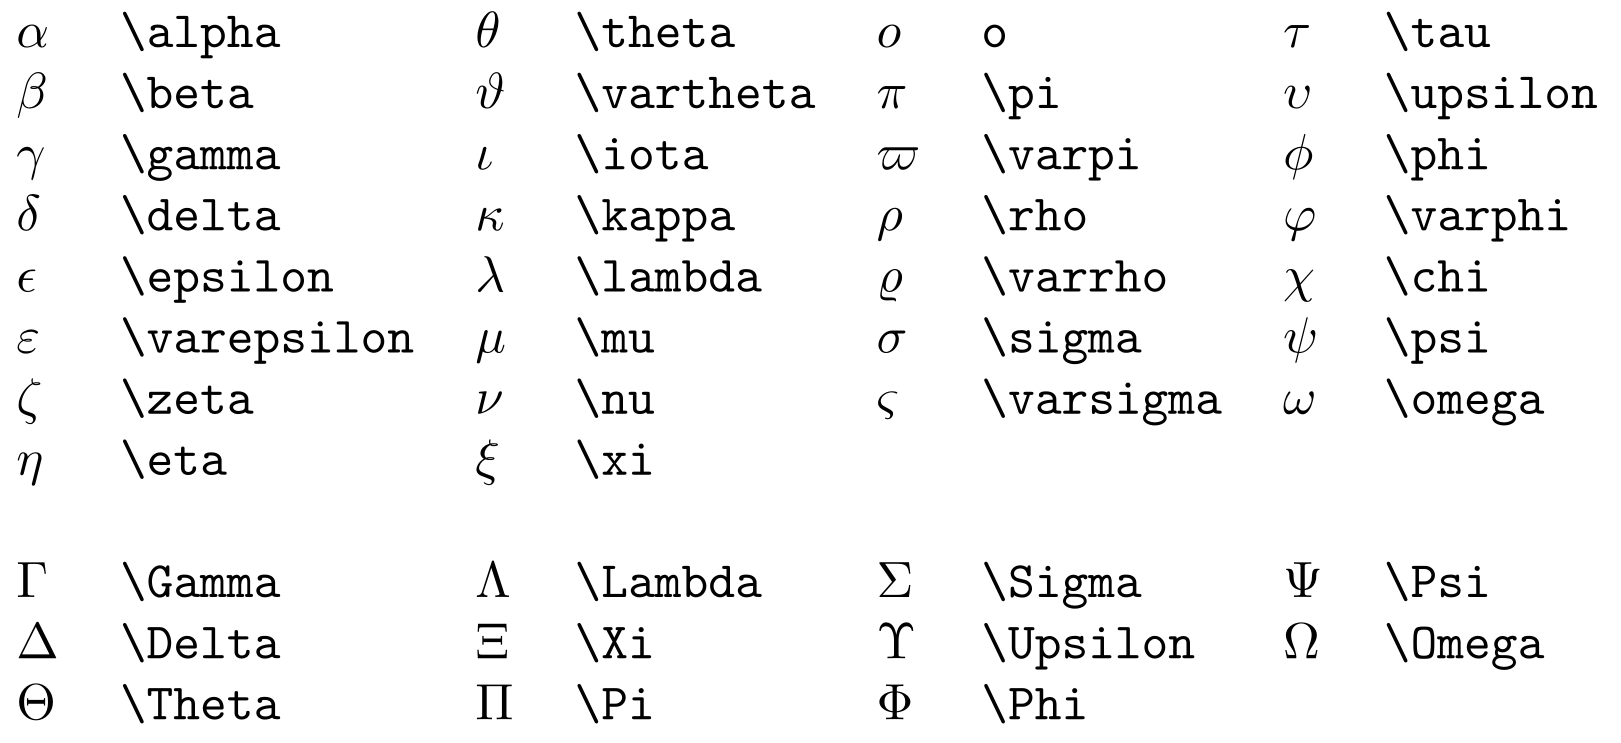
\includegraphics[width = \textwidth]{greek.png}
\end{center}


\subsection{\AmS{} packages}

The amsmath package enhances the capabilities of LaTeX for mathematical typesetting. It provides various environments for aligning equations, creating multiline equations, and more.

For all environments please read through \href{http://mirrors.ctan.org/macros/latex/required/amsmath/amsldoc.pdf}{documentation}.

\subsubsection{Environments}
There are some important environments to encapsulate mathematics: equation, gather and align.

\begin{itemize}
    \item[\textbf{Equation}] If you want to include an equation in display-style math mode, use the equation environment. The syntax is: 
    \begin{verbatim}
\begin{equation}
    n > \frac{1}{2} + \sqrt{2m\log\left(\frac{1}{1-p}\right)+\frac{1}{4}}
\end{equation}
    \end{verbatim}
\begin{equation}
    n > \frac{1}{2} + \sqrt{2m\log\left(\frac{1}{1-p}\right)+\frac{1}{4}}
\end{equation}

\item[\textbf{Align}] If you have multiple equations, the align environment aligns equations based on the \verb|&| delimiter. An example below: 
\begin{verbatim}
\begin{align}
    a^4 + 4b^4 &= (a^2+2b^2)^2 - 2(a^2)(2b^2) \nonumber \\
    \tag{Sophie Germain Identity}
               &= (a^2 - 2ab + 2b^2)(a^2 + 2ab +2b^2)    
\end{align}
\end{verbatim}
\begin{align}
    a^4 + 4b^4 &= (a^2+2b^2)^2 - 2(a^2)(2b^2) \nonumber \\
    \tag{Sophie Germain Identity}
               &= (a^2 - 2ab + 2b^2)(a^2 + 2ab +2b^2)    
\end{align}
\item[\textbf{Gather}] This environment aligns multiple equations to the centre of the text width. An example :
\begin{verbatim}
\begin{gather*}
    F_n = F_{n-1} + F_{n-2} \\ 
    F_n = \frac{\left(\frac{1+\sqrt{5}}{2}\right)^n - 
    \left(\frac{1-\sqrt{5}}{2}\right)^n}{\sqrt{5}}
\end{gather*}
\end{verbatim}
\begin{gather*}
    F_n = F_{n-1} + F_{n-2} \\ 
    F_n = \frac{\left(\frac{1+\sqrt{5}}{2}\right)^n - \left(\frac{1-\sqrt{5}}{2}\right)^n}{\sqrt{5}}
\end{gather*}
\end{itemize}
\subsubsection{AMS Fonts}
% show mathcal and mathbb fonts
\paragraph{Math Symbols} We use multiple symbols in math and physics.

\(\mathcal{L}: \text{Lagrangian} \quad \mathbb{I}_n : \text{Identity Matrix of dimension } n\)

\(\mathfrak{I} : \text{Imaginary Part of a complex number}\)

\subsection{Physics Package}
The physics package is just a list of macros to make writing physics and math easier, i.e. less cumbersome notation. \cite{demaine2023author}

For better understanding of these commands read through the \href{http://mirrors.ctan.org/macros/latex/contrib/physics/physics.pdf}{documentation}.

\subsubsection{Automatic bracing}

This is very helpful when you write complicated math equations.
\[
\textsf{A} = (\frac{\textsf{A} + \textsf{A}^\top}{2}) + (\frac{\textsf{A} - \textsf{A}^\top}{2}) \quad ; \quad \textsf{A} = \qty(\frac{\textsf{A} + \textsf{A}^\top}{2}) + \qty(\frac{\textsf{A} - \textsf{A}^\top}{2})
\]

\subsubsection{Vectors}
Vectors are typically represented in two ways in books using vector-bold notation or accenting it with an arrow or the unit vectors. Here are both of them: 
\begin{itemize}
    \item \verb|\vb{a} | \(\rightarrow \vb{a}\). However, this does not work for Greek symbols, so instead of using \verb|\vb{}|,\verb|\vb*{}| needs to be used. However, that also italicizes your letter.  \\ For example \verb|\vb*{\theta} | \(\rightarrow \vb*{\theta}\). However it does not italicize Capital Greek Letters eg: \verb|\vb*{\theta} | \(\rightarrow \vb*{\Theta}\). 
    \item \verb|\va{a} | \(\rightarrow \va{a}\). The same conditions apply to Greek Letters.
    \item \verb|\vu{a} | \(\rightarrow \vu{a}\). This can also be done using the \verb|\hat{}| command, which gives \( \hat{a}\).
\end{itemize}
\subsubsection{Derivatives or Partial Derivatives}
Partial Derivatives have very useful macros when it comes to the physics package. Here are some syntaxes with certain arguments for differential calculus.
\begin{itemize}
    \item[\textbf{Derivative}] The standard derivative in Leibniz Notation is written like \verb|\dv{x}|\(\rightarrow\dv{x}\). Here are certain variations of it:
    \begin{itemize}
        \item \verb|\dv{f}{x}| \(\rightarrow \dv{f}{x}\)
        \item \verb|\dv[n]{y}{x}|\(\rightarrow \dv[n]{y}{x}\)
    \end{itemize}
    We can also write in Newton's Notation using 
    \verb|\dot{x}|\(\rightarrow\dot{x}\). And we have \verb|\ddot{x}|\(\rightarrow\ddot{x}\).
    \item[\textbf{Partial Dv.}] We write partial derivatives with some variations in the following syntaxes:
    \begin{itemize}
        \item \verb|\pdv{x}| \(\rightarrow\pdv{x}\)
        \item \verb|\pdv{f}{x}| \(\rightarrow\pdv{f}{x}\)
        \item \verb|\pdv[n]{f}{x}| \(\rightarrow\pdv[n]{f}{x}\)
        \item \verb|\pdv{f}{x}{y}| \(\rightarrow\pdv{f}{x}{y}\)
        \item \verb|\pdv*{f}{y}| \(\rightarrow\pdv*{f}{y}\)
    \end{itemize}
    \item[\textbf{Vector Calc.}] The following syntaxes are useful to define most differential vector calculus.
    \begin{itemize}
        \item[\textbf{Grad}] \verb|\grad{A}|\( \rightarrow \grad{A}\)
        \item[\textbf{Divergence}] \verb|\div{\vb{A}}|\( \rightarrow \div{\vb{A}}\)
        \item[\textbf{Curl}] \verb|\curl{\vb{A}}|\( \rightarrow \curl{\vb{A}}\) 
        \item[\textbf{Laplacian}] \verb|\laplacian{A}|\( \rightarrow \laplacian{A}\)
    \end{itemize}
\end{itemize}
Here is a simple example of the use case of the physics package:
\begin{align*}
    \div{\va{E}} &= \frac{\rho}{\epsilon_0}\\
    \div{\va{B}} &= 0 \\
    \curl{\va{E}} &= -\pdv{\va{B}}{t}\\
    \curl{\va{B}} &= \mu_0\va{J}+\frac{1}{c^2} \pdv{\va{E}}{t}
\end{align*}
\subsubsection{Matrices}

For writing matrices, \verb|physics| package provides simple commands like we can write \textsc{Vandermonde Matrix}
\begin{verbatim}
\mqty(
1 & 1 & 1 & \cdots & 1 \\
x_0 & x_1 & x_2 & \cdots & x_n \\
x_0^2 & x_1^2 & x_2^2 & \cdots & x_n^2 \\
\vdots & \vdots & \vdots &  & \vdots \\
x_0^n & x_1^n & x_2^n & \cdots & x_n^n
)
\end{verbatim}
\[
\mqty|
1 & 1 & 1 & \cdots & 1 \\
x_0 & x_1 & x_2 & \cdots & x_n \\
x_0^2 & x_1^2 & x_2^2 & \cdots & x_n^2 \\
\vdots & \vdots & \vdots &  & \vdots \\
x_0^n & x_1^n & x_2^n & \cdots & x_n^n
|
\]

\section{Images, Floats, Captions}

In LaTeX, figures (images) are typically handled as floats. Floats are containers for things in a document that cannot be broken over a page. They are "floated" to a location, such as the top or bottom of a page, and can include images, tables, and other similar elements.

\begin{verbatim}
\begin{figure}[H]
    \centering
    \includegraphics[width=0.48\textwidth]{guatam-lol.jpeg}
    \caption{Gautam Singh (22MS023) CP}
    \label{fig:gautam}
\end{figure}
\end{verbatim}

\begin{figure}[H]
    \centering
    
\includegraphics[width=0.48\textwidth]{gautam-lol.png}
    \caption{Gautam Singh (22MS023) CP}
    \label{fig:gautam}
\end{figure}

\subsection{Adding Multiple Images}

To add multiple images in LaTeX, you can use the \verb|subfigure| environment from the \verb|subcaption| package.

\begin{verbatim}
\begin{figure}[H]

\begin{subfigure}{0.5\textwidth}
\centering
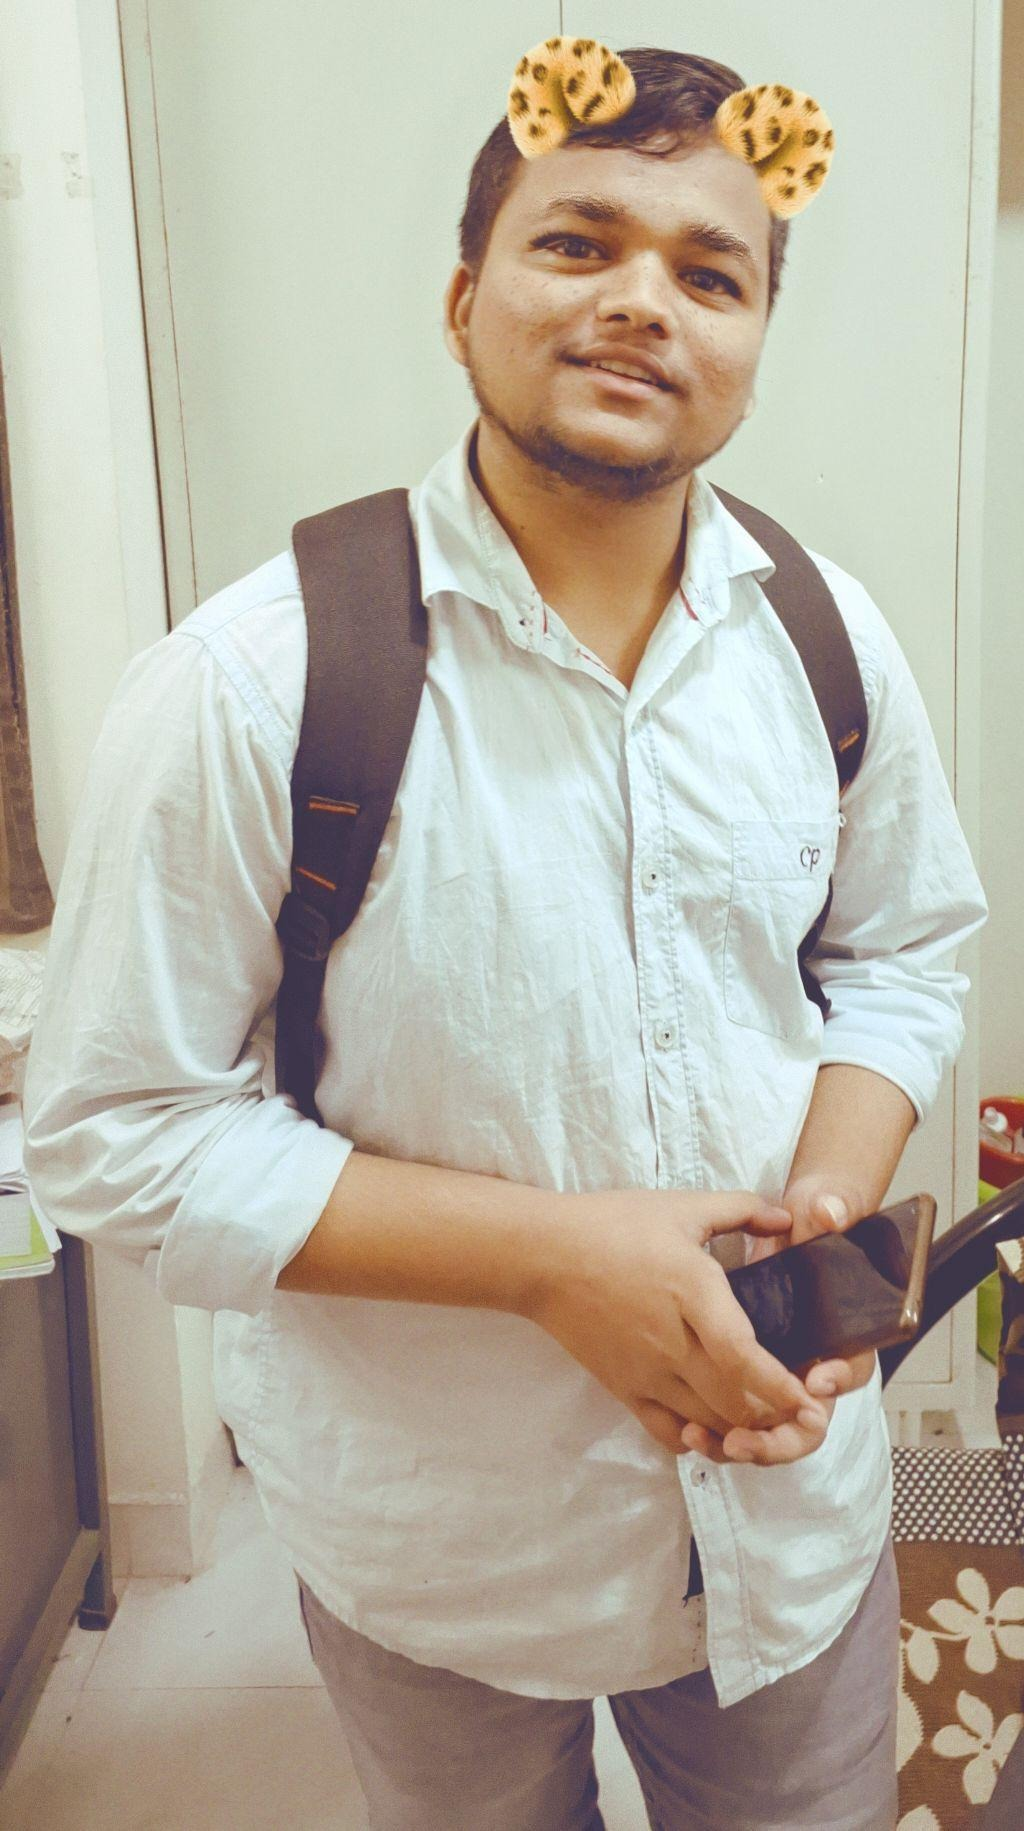
\includegraphics[scale=0.12]{vikash-lol.jpeg} 
\caption{Vikash Kumar (22MS036) \cite{gato2011schroedingers}}
\label{fig:vikash}
\end{subfigure}
\begin{subfigure}{0.5\textwidth}
\centering
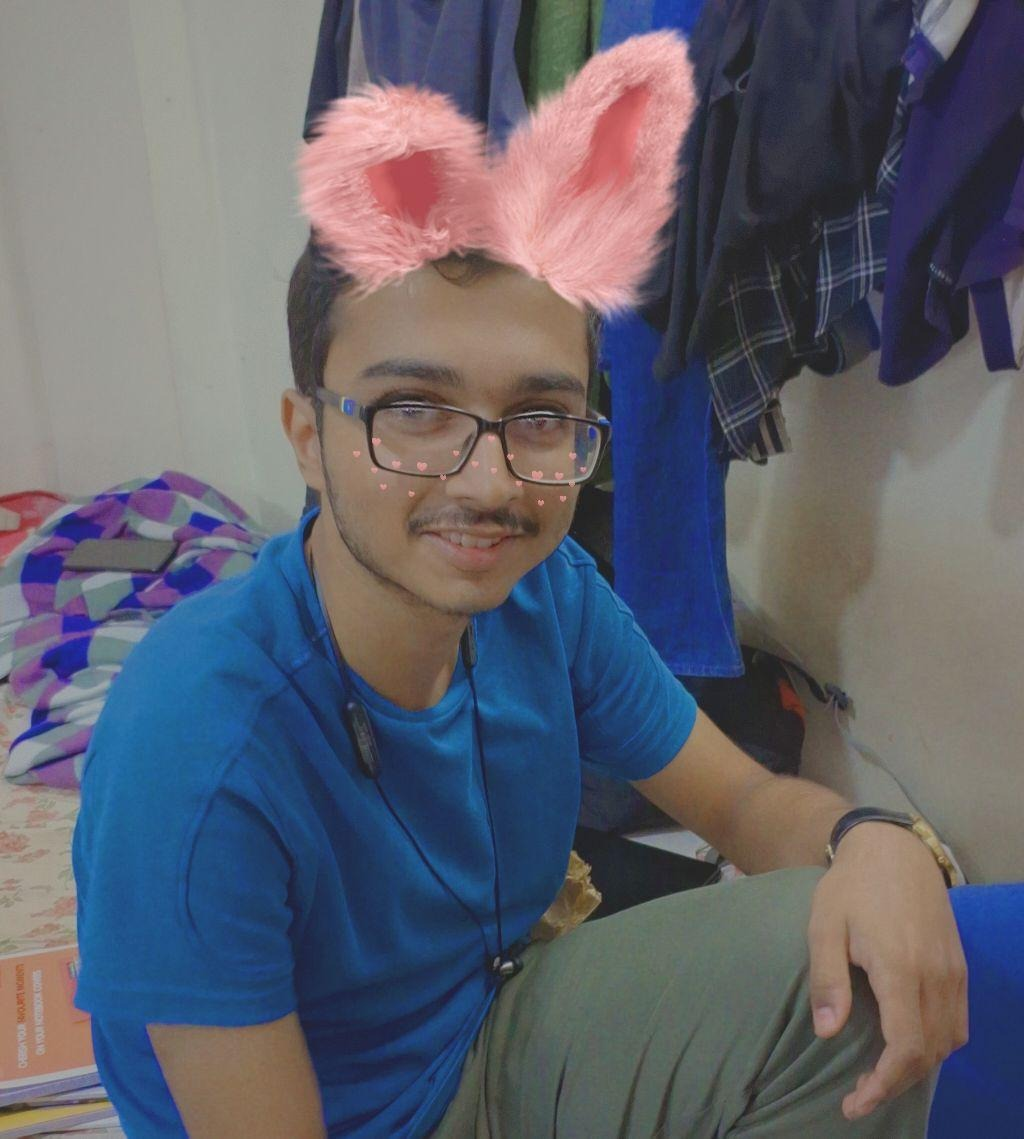
\includegraphics[width=0.9\linewidth]{ronit-lol.jpeg}
\caption{Ronit Bhuyan (22MS025)}
\label{fig:ronit}
\end{subfigure}

\begin{subfigure}{0.5\textwidth}
\centering
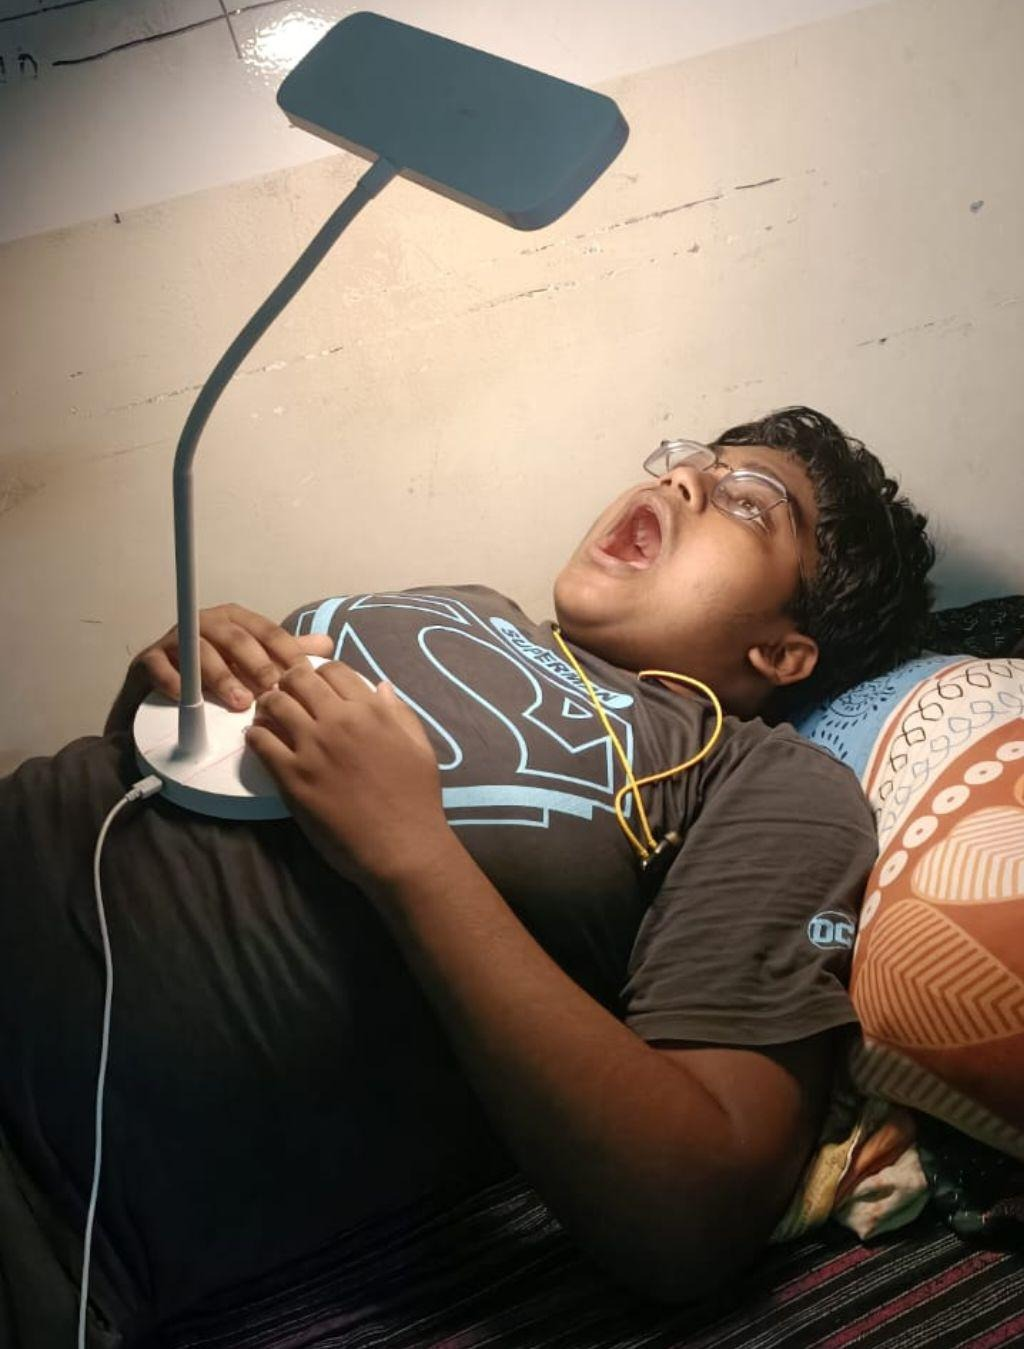
\includegraphics[width = 0.9\linewidth]{sabarno-lol.jpeg}
\caption{Sabarno Saha (22MS037)}
\label{fig:sabarno}
\end{subfigure}
\begin{subfigure}{0.5\textwidth}
\centering
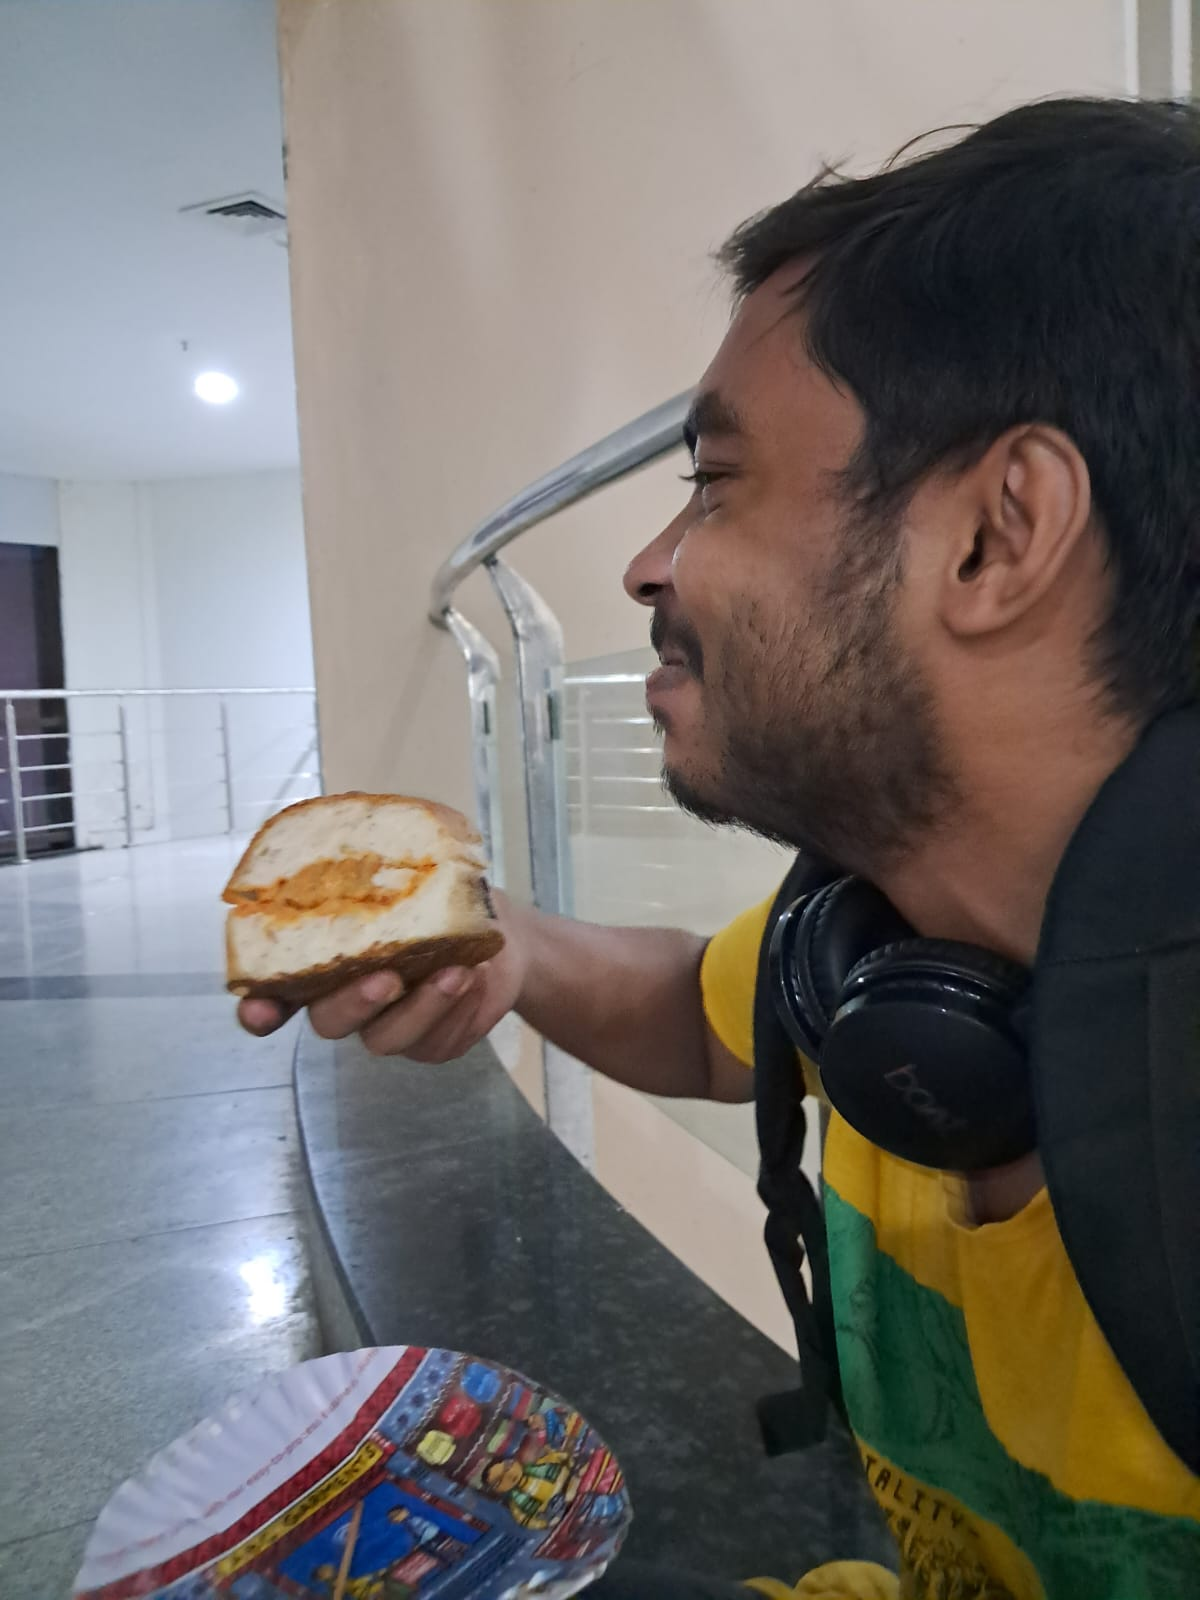
\includegraphics[width=0.9\linewidth]{debayan-lol.jpeg}
\caption{Debayan Sarkar (22MS002)}
\label{fig:debayan}
\end{subfigure}

\caption{People who helped in this handout}
\label{fig:multipleImg}
\end{figure}
\end{verbatim}

\noindent Here we will discuss how to refer this images:
\begin{verbatim}
You can reference individual subfigures using \autoref{fig:vikash} and 
\autoref{fig:sabarno}. The overall figure is referenced using 
\autoref{fig:multipleImg}.
\end{verbatim}
You can reference individual subfigures using \autoref{fig:vikash} and \autoref{fig:sabarno}. The overall figure is referenced using \autoref{fig:multipleImg}.

\begin{figure}[H]

\begin{subfigure}{0.5\textwidth}
\centering
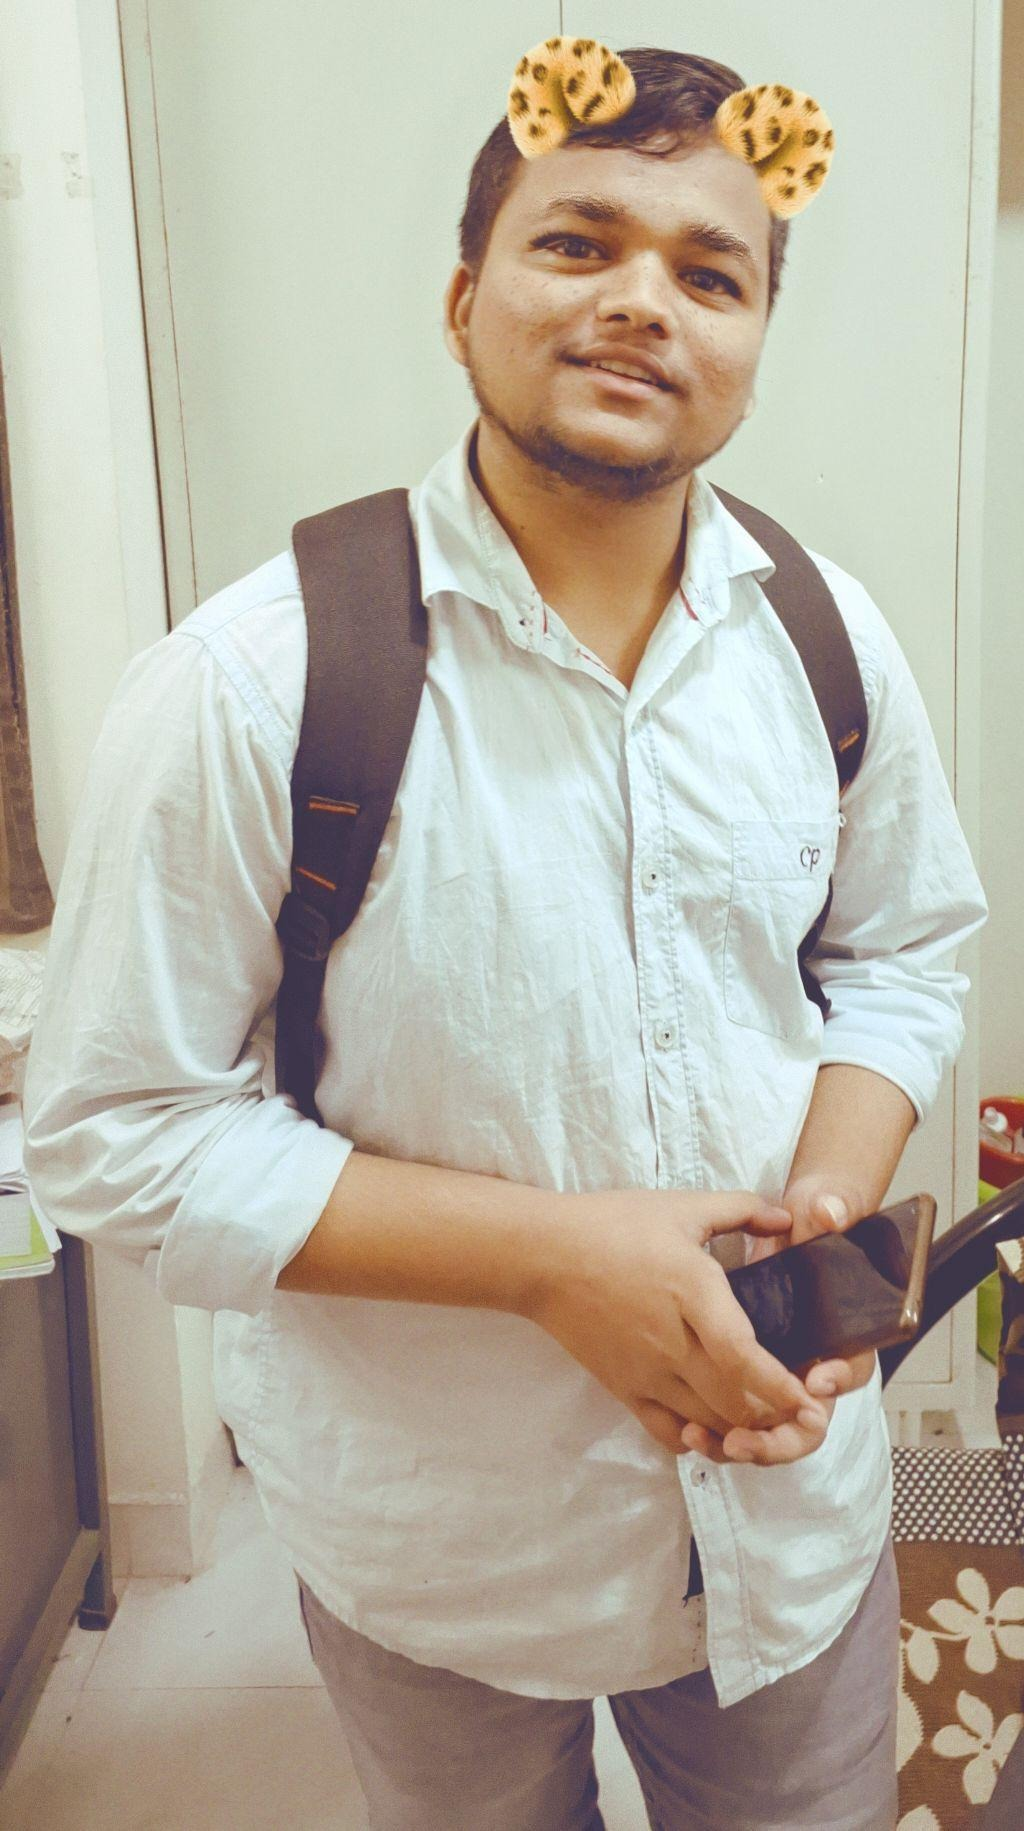
\includegraphics[scale=0.12]{vikash-lol.jpeg} 
\caption{Vikash Kumar (22MS036) \cite{gato2011schroedingers}}
\label{fig:vikash}
\end{subfigure}
\begin{subfigure}{0.5\textwidth}
\centering
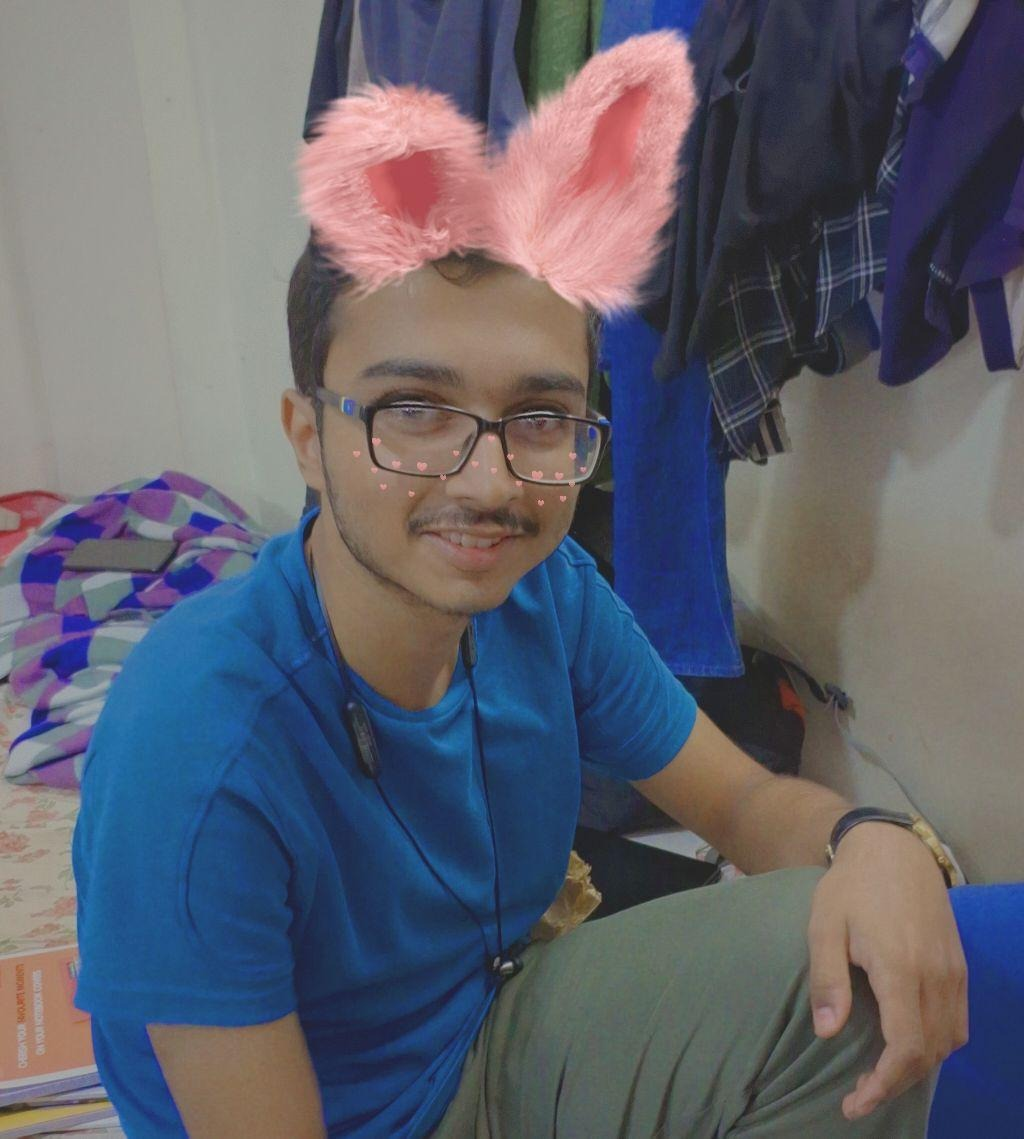
\includegraphics[width=0.9\linewidth]{ronit-lol.jpeg}
\caption{Ronit Bhuyan (22MS025)}
\label{fig:ronit}
\end{subfigure}

\begin{subfigure}{0.5\textwidth}
    \centering
    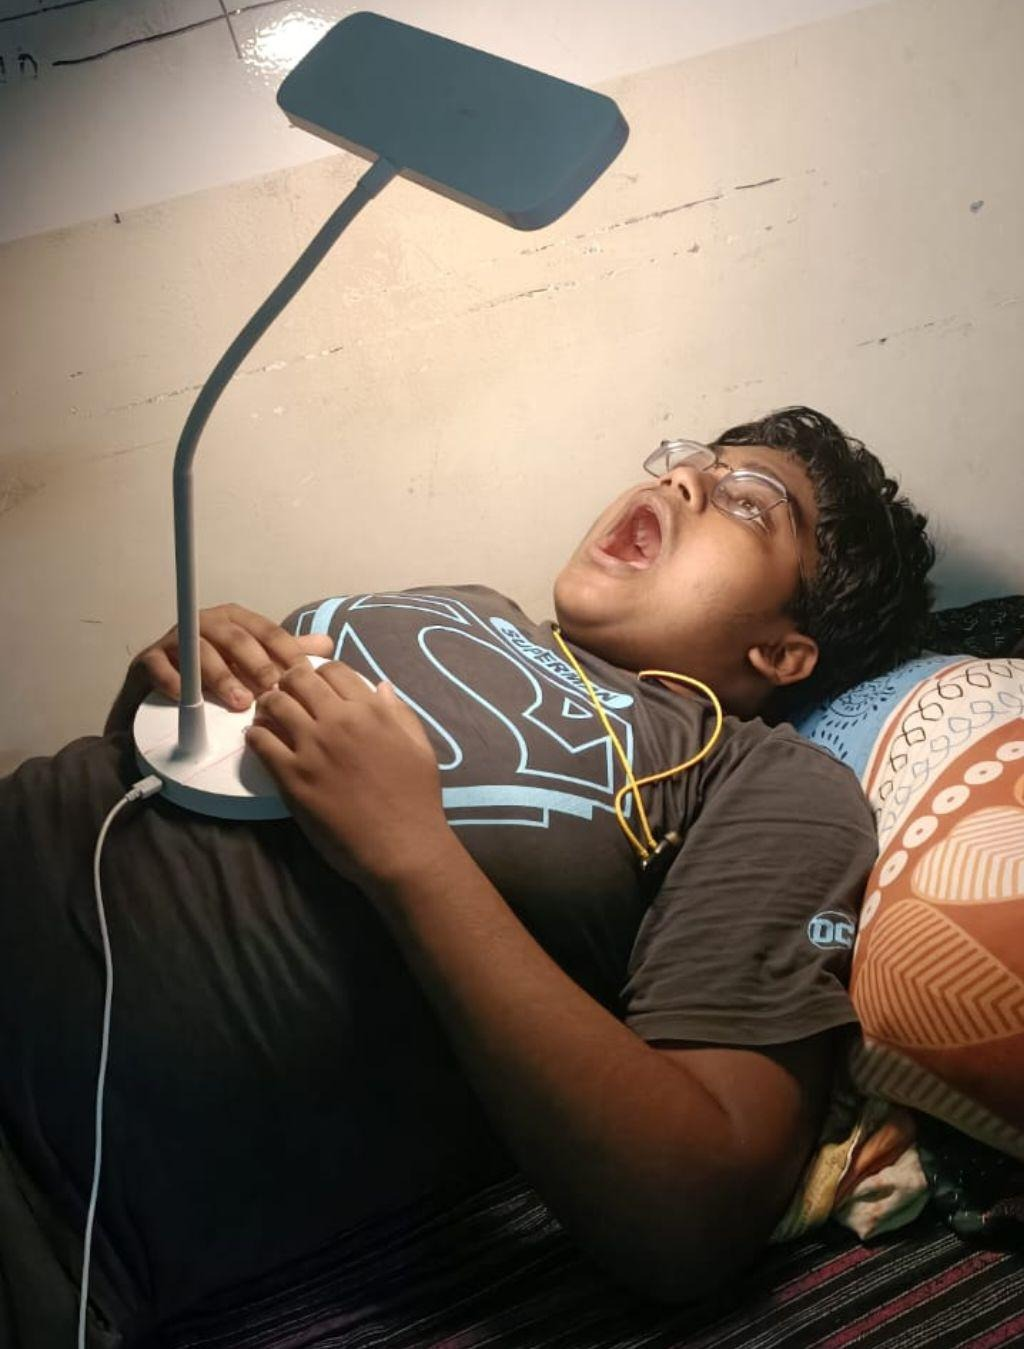
\includegraphics[width = 0.9\linewidth]{sabarno-lol.jpeg}
    \caption{Sabarno Saha (22MS037)}
    \label{fig:sabarno}
\end{subfigure}
\begin{subfigure}{0.5\textwidth}
\centering
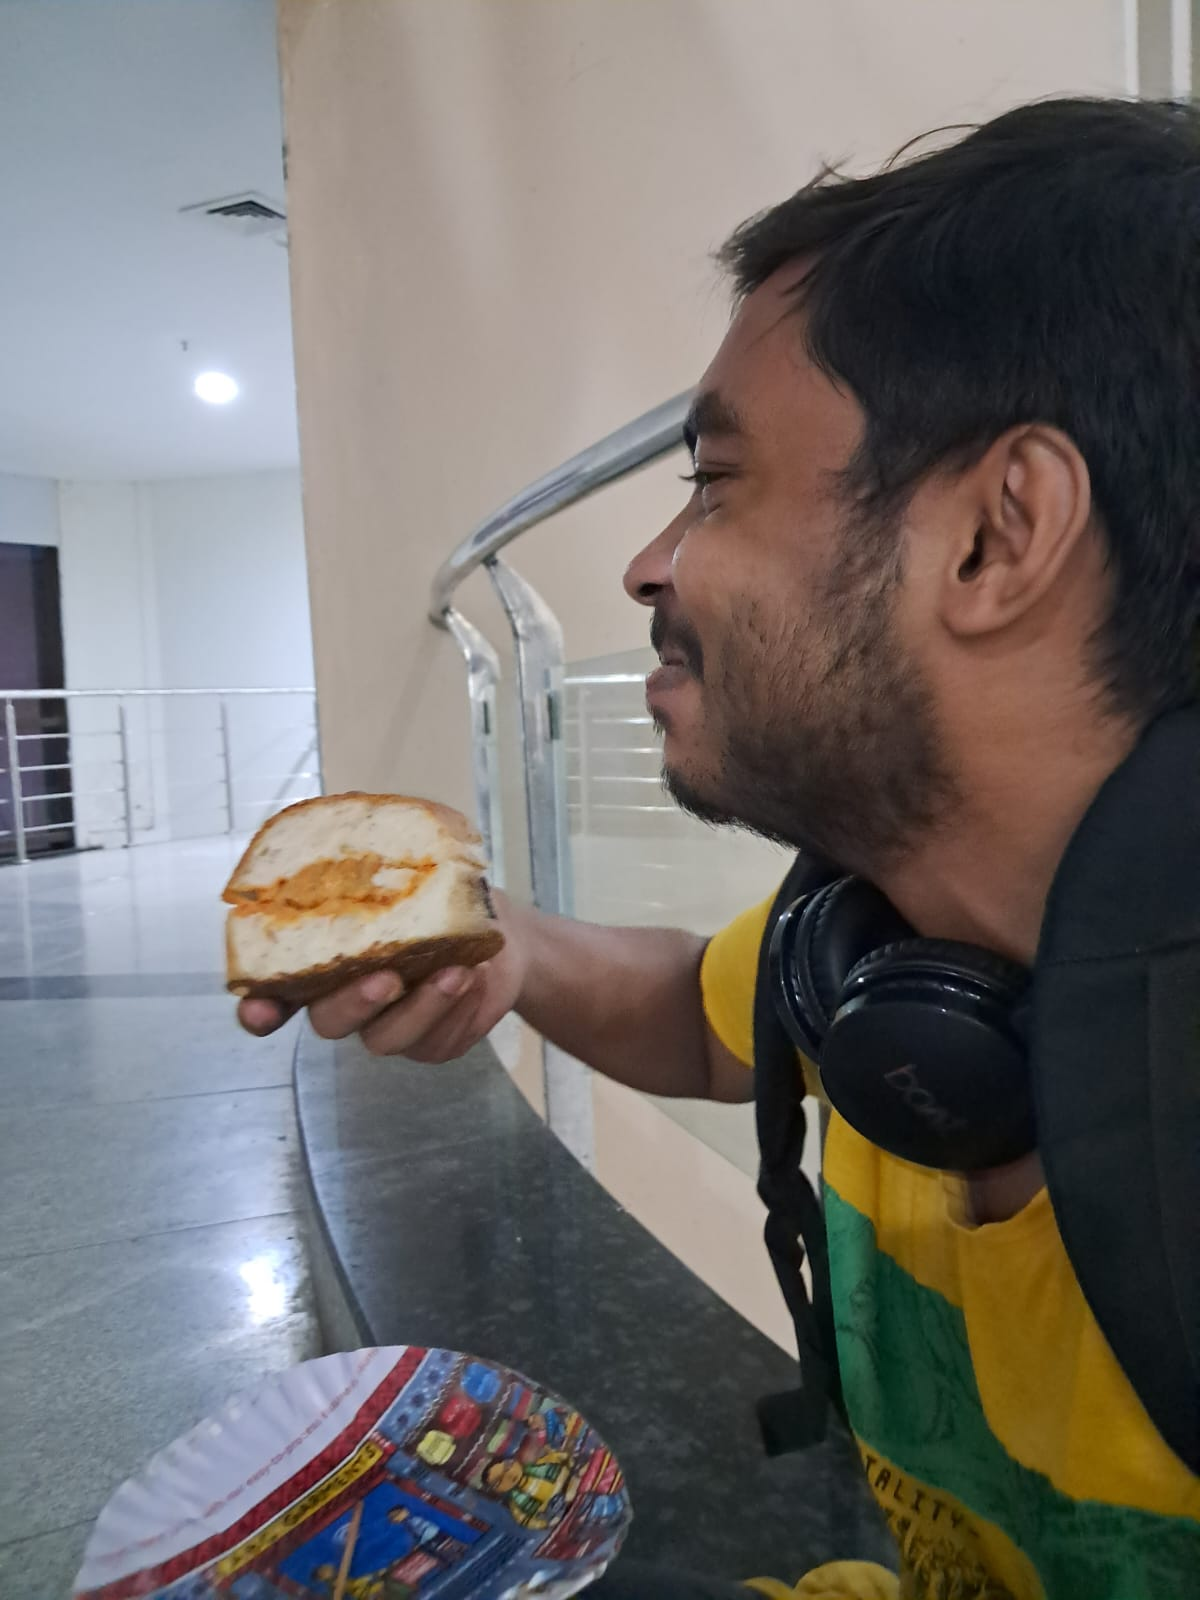
\includegraphics[width=0.9\linewidth]{debayan-lol.jpeg}
\caption{Debayan Sarkar (22MS002)}
\label{fig:debayan}
\end{subfigure}

\caption{People who helped in this handout}
\label{fig:multipleImg}
\end{figure}

\section{Lists}
\subsection{Unordered List}
To create unordered lists in \LaTeX{}, one can use the \texttt{itemize} environment. Individual items are added using the \verb|\item| command. Shown below is an easy example of how to create unordered (bulleted) lists:
\begin{verbatim}
\begin{itemize}
    \item Diane
    \item Todd
    \item Carolyn
    \item[\textbf{Sarah}] Lynn
\end{itemize}
\end{verbatim}
\begin{itemize}
    \item Diane
    \item Todd
    \item Carolyn
    \item[\textbf{Sarah}] Lynn
\end{itemize}
\subsection{Ordered List}
One can create Ordered Lists using the \texttt{enumerate} environment. Again, each item in the list is created using the \verb|\item| command. Below is a simple example showing the same:
\begin{verbatim}
    \begin{enumerate}
        \item Ted
        \item Barney
        \item Robin
        \item Lilly
        \item Marshall
    \end{enumerate}
\end{verbatim}
\begin{enumerate}
    \item Ted
    \item Barney
    \item Robin
    \item Lilly
    \item Marshall
\end{enumerate}
\subsection{Nested Lists}
Sometimes, you may want to create lists inside lists. To create one in \LaTeX, you do just that! i.e., create another \texttt{enumerate} environment inside the existing one. Here's an example:
\begin{verbatim}
    \begin{enumerate}
        \item King
        \item S-Class
        \begin{enumerate}
            \item Blast
            \item Tornado
        \end{enumerate}
        \item A-Class
        \begin{enumerate}
            \item Sweet Mask
            \item Caped Baldy
        \end{enumerate}
    \end{enumerate}
\end{verbatim}
\begin{enumerate}
    \item King
    \item S-Class
    \begin{enumerate}
        \item Blast
        \item Tornado
    \end{enumerate}
    \item A-Class
    \begin{enumerate}
        \item Sweet Mask
        \item Caped Baldy
    \end{enumerate}
\end{enumerate}
\subsection{Custom Labels}
Sometimes, you may not want to use the default symbols or numberings for the labels in the lists. You may want to customize them. You can also do that in \LaTeX\, using the \texttt{enumitem} package. For instance, if you're typing out some questions and you want the questions to be labelled as Q1, Q2, and so on instead of the default 1,2, etc., you could do this:
\begin{verbatim}
    \begin{enumerate}[label=Q\arabic*.]
        \item This is question 1.
        \item This is question 2.
    \end{enumerate}
\end{verbatim}
\begin{enumerate}[label=Q\arabic*.]
    \item Let $a$ and $b$ be two positive integers such that $ab + 1$ divides $ab + 1$. Show that $\cfrac{a^2 + b^2}{ab + 1}$ is the square of an integer.
    \item Show that every even integer can be written as the sum of two primes.
\end{enumerate}
\section{Table}
This is the simplest way to create a table in \LaTeX\ using the \texttt{tabular} environment:
    \begin{verbatim}
    \begin{center}
    \begin{tabular}{ c c c }
     cell1 & cell2 & cell3 \\ 
     cell4 & cell5 & cell6 \\  
     cell7 & cell8 & cell9    
    \end{tabular}
    \end{center}
    \end{verbatim}
\begin{center}
\begin{tabular}{ c c c }
 cell1 & cell2 & cell3 \\ 
 cell4 & cell5 & cell6 \\  
 cell7 & cell8 & cell9    
\end{tabular}
\end{center}
\subsection{Column and Row borders}
However, as you can see, this doesn't have column borders. The \texttt{\{c c c\}} implies that the table generated will have three columns, without any column borders, and the text will be centre-aligned in each of the cells. The cell contents are separated by \texttt{\&}, and the rows are separated by \verb|\\|. To create a table with column borders, you can use \texttt{\{| c | c | c |\}} as shown below:
    \begin{verbatim}
\begin{center}
\begin{tabular}{| c | c | c |}
 cell1 & cell2 & cell3 \\ 
 cell4 & cell5 & cell6 \\  
 cell7 & cell8 & cell9    
\end{tabular}
\end{center}
    \end{verbatim}
\begin{center}
\begin{tabular}{| c | c | c |}
 cell1 & cell2 & cell3 \\ 
 cell4 & cell5 & cell6 \\  
 cell7 & cell8 & cell9    
\end{tabular}
\end{center}
Still, there aren't any row borders. To add those, you can add \verb|\hline| in the appropriate line. An example is shown below:
    \begin{verbatim}
\begin{center}
\begin{tabular}{| c | c | c |}
\hline
cell1 & cell2 & cell3 \\ 
\hline
cell4 & cell5 & cell6 \\  
\hline
cell7 & cell8 & cell9 \\   
\hline
\end{tabular}
\end{center}
    \end{verbatim}
\begin{center}
\begin{tabular}{| c | c | c |}
\hline
 cell1 & cell2 & cell3 \\ 
 \hline
 cell4 & | & || \\  
 \hline
 cell7 & || & |\_ \\   
 \hline
\end{tabular}
\end{center}
\subsection{Merged Rows and Columns}
You may want to merge some rows or columns. In other words, you may want some cells to span across multiple rows/columns. You can do that after including the \texttt{multirow} package in the preamble, as shown in the example below:
\begin{verbatim}
\begin{table}[h]
    \centering
    \begin{tabular}{ |c|c|c| } 
        \hline
        col1 & col2 & col3 \\
        \hline
        \multicolumn{2}{ | c | }{Spans 2 columns} & no span \\
        \hline
        \multirow{3}{3em}{Spans 2 rows} & cell2 & cell3 \\ 
        & cell5 & cell6 \\ 
        & cell8 & cell9 \\ 
        \hline
    \end{tabular}
    \caption{This is a table caption}
    \label{Table:merge}
\end{table}
\end{verbatim}
\begin{table}[h]
\centering
\begin{tabular}{ |c|c|c| } 
\hline
col1 & col2 & col3 \\
\hline
\multicolumn{2}{ | c | }{Spans 2 columns} & no span \\
\hline
\multirow{3}{3em}{Spans 2 rows} & cell2 & cell3 \\ 
& cell5 & cell6 \\ 
& cell8 & cell9 \\ 
\hline
\end{tabular}
\caption{This is a table caption}
\label{Table:merge}
\end{table}
This also adds a caption and a label to the table using the \texttt{table} environment.

That ends our discussion on the basics of \LaTeX{} tables.
With some further styling, you can create stuff like this.
\begin{center}
    \begin{tabular}{| c | c |}
    \hline
    \multicolumn{2}{| c |}{Method of undetermined coefficients} \\
    \hline \hline
         $f_i(t)$ & $y_{p_i}$ \\
         \hline \hline
         $Ke^{at}$ & $ke^{at}$ \\
         \hline
         $Kt^m$ & $k_mt^m + k_{m-1}t^{m-1} + \cdot \cdot \cdot + k_0$\\
         \hline
         $K\cos(bt)$ or $K\sin(bt)$ & $k_1 \sin (bt) + k_2 \cos(bt)$\\
         \hline
         $Ke^{at} \sin (bt)$ or $Ke^{at} \cos(bt)$ & $e^{at}(k_1 \sin (bt) + k_2 \cos(bt))$ \\
         \hline 
         $Kt^me^{at}$ & $e^{at}(k_mt^m + k_{m-1}t^{m-1} + \cdot \cdot \cdot + k_0)$\\
         \hline
         $Kt^m \cos(bt)$ or $Kt^m \sin(bt)$ & $(k_mt^m + \cdot \cdot \cdot + k_0)(a_1 \sin (bt) + a_2 \cos(bt))$\\
         \hline
    \end{tabular}
\end{center}


\section{Adding Bibliography}

As there are multiple methodologies to add \textsc{Bibliography}, we have decided to go with Biber backend and Biblatex as formatting packages for this discussion. The other options are the Bibtex backend and natbib package\cite{timokhin2020novel}. Adding a bibliography is a very big discussion, so we recommend you go through: \href{https://www.overleaf.com/learn/latex/Bibliography_management_with_biblatex}{overleaf blog}. Or for a detailed introduction, read through \href{https://www.mn.uio.no/ifi/tjenester/it/hjelp/latex/biblatex-guide.pdf}{biblatex guide}.

And to better understand the decision we made, please go through this \href{https://tex.stackexchange.com/a/25702}{Stack Exchange} answer.


\section{Extra Useful Packages}

\subsection{Geometry}

The \verb|geometry| package in \LaTeX{} is a powerful tool that allows users to customize the layout of their documents by adjusting page dimensions, margins, and other related parameters. It provides a convenient interface for controlling the overall geometry of a page.

To get very good idea of useability of this package read through the \href{http://mirrors.ctan.org/macros/latex/contrib/geometry/geometry.pdf}{documentation}.

\begin{verbatim}
\usepackge{geometry}

---

\geometry{left=1in, right=1in, top=1in, bottom=1in}
\end{verbatim}

\subsection{Hyperref}

The \verb|hyperref| package is a powerful tool in \LaTeX{} that allows you to create hyperlinks within your documents. It is commonly used for adding hyperlinks to sections, figures, citations, URLs, and internal references. The hyperref package also provides options for customizing the appearance of links and other interactive features.

To get very good idea of useability of this package read through the \href{http://mirrors.ctan.org/macros/latex/contrib/hyperref/doc/hyperref-doc.pdf}{documentation}.

\subsubsection{Hyperlinks}

The \verb|\href{URL}{text}| command is used to create hyperlinks. For example:
\begin{verbatim}
\href{https://www.example.com}{Visit our website}
\end{verbatim}
\href{https://youtu.be/xvFZjo5PgG0?si=sYAoYo_DIapgCkSn}{Visit our website}

The \verb|\url{}| command is available for typesetting URLs, and hyperref allows you to customize the appearance of these links:
\begin{verbatim}
\url{gnu.org}
\end{verbatim}
\url{gnu.org}

\subsubsection{Cross Referencing}

hyperref provides commands like \verb|\autoref|, \verb|\nameref| and \verb|\ref| that automatically generate the appropriate prefix for cross-references. For example:
\begin{verbatim}
This is an example \autoref{Table:merge}. And this works \nameref{Table:merge}.
\end{verbatim}
This is an example \autoref{Table:merge}. And this works \nameref{Table:merge}.

\subsubsection{PDF Metadata}

The hyperref package allows you to set metadata for the PDF file, such as the title, author, and keywords:
\begin{verbatim}
\hypersetup{
    pdftitle={LaTeX Handout Slashdot},
    pdfauthor={Piyush, Sabarno, Debayan, Gautam},
    pdfsubject={Slashdot},
    pdfkeywords={handout, latex, slashdot},
    pdfpagemode=FullScreen,
}
\end{verbatim}

\subsubsection{Customizing Link Colors}

You can customize the color of hyperlinks using the \texttt{colorlinks} option and related options such as \texttt{linkcolor}, \texttt{citecolor}, and \texttt{urlcolor}:
\begin{verbatim}
\hypersetup{
    draft = false,
    linktocpage = true,
    colorlinks=true,
    linkcolor=DeepSkyBlue4,
    filecolor=magenta,      
    urlcolor=teal,
    citecolor=Green4,
}
\end{verbatim}

\subsection{tcolorbox, mdframed}

\subsection{tikz, pgfplots}
An example using Tikz:
\begin{verbatim}
\tikzset{every picture/.style={line width=0.75pt}} %set default line 
width to 0.75pt        

\begin{center}
    
\begin{tikzpicture}[x=0.75pt,y=0.75pt,yscale=-1,xscale=1]
%uncomment if require: \path (0,300); %set diagram left start at 0,
and has height of 300

%Straight Lines [id:da5022345784814793] 
\draw    (170,158.81) -- (203.13,158.42) ;
%Straight Lines [id:da015487184503324869] 
\draw    (486.86,159.97) -- (519.99,159.58) ;
%Shape: Inductor (Air Core) [id:dp6825263183809437] 
\draw   (203.13,159.97) -- (228.66,159.97) .. 
controls (229.03,155.88) and (232.58,152.38) .. 
(237.59,151.15) .. controls (242.61,149.93) and 
(248.08,151.23) .. (251.36,154.43) .. 
controls (253.9,156.93) and (254.93,160.16) .. (254.2,163.3) .. 
controls (254.2,164.52) and (252.93,165.51) .. 
(251.36,165.51) .. controls (249.8,165.51) and 
(248.53,164.52) .. 
(248.53,163.3) .. controls (247.8,160.16) and (248.83,156.93) .. 
(251.36,154.43) .. controls (254.31,151.77) and (258.42,150.26) .. 
(262.71,150.26) .. controls (267.01,150.26) and (271.11,151.77) .. 
(274.06,154.43) .. controls (276.6,156.93) and (277.63,160.16) .. 
(276.9,163.3) .. controls (276.9,164.52) and (275.63,165.51) .. 
(274.06,165.51) .. controls (272.5,165.51) and (271.22,164.52) ..
(271.22,163.3) .. controls (270.49,160.16) and (271.53,156.93) .. 
(274.06,154.43) .. controls (277.01,151.77) and (281.12,150.26) .. 
(285.41,150.26) ..
controls (289.71,150.26) and (293.81,151.77) .. (296.76,154.43) ..
controls (299.3,156.93) and (300.33,160.16) .. (299.6,163.3) .. 
controls (299.6,164.52) and (298.33,165.51) .. (296.76,165.51) ..
controls (295.2,165.51) and (293.92,164.52) .. (293.92,163.3) .. 
controls (293.19,160.16) and (294.23,156.93) .. (296.76,154.43) .. 
controls (300.05,151.23) and (305.51,149.93) .. (310.53,151.15) .. 
controls (315.55,152.38) and (319.09,155.88) .. (319.46,159.97) 
-- (345,159.97) ;
%Shape: Inductor (Air Core) [id:dp8148657217032366] 
\draw   (345,159.97) -- (370.53,159.97) .. controls (370.9,155.88)
and (374.44,152.38) .. (379.46,151.15) .. controls (384.48,149.93)
and (389.94,151.23) .. (393.23,154.43) .. controls (395.77,156.93)
and (396.8,160.16) .. (396.07,163.3) .. controls (396.07,164.52)
and (394.8,165.51) .. (393.23,165.51) .. controls (391.67,165.51)
and (390.39,164.52) .. (390.39,163.3) .. controls (389.66,160.16)
and (390.7,156.93) .. (393.23,154.43) .. controls (396.18,151.77)
and (400.29,150.26) .. (404.58,150.26) .. controls (408.88,150.26)
and (412.98,151.77) .. (415.93,154.43) .. controls (418.46,156.93)
and (419.5,160.16) .. (418.77,163.3) .. controls (418.77,164.52)
and (417.5,165.51) .. (415.93,165.51) .. controls (414.36,165.51)
and (413.09,164.52) .. (413.09,163.3) .. controls (412.36,160.16)
and (413.4,156.93) .. (415.93,154.43) .. controls (418.88,151.77)
and (422.98,150.26) .. (427.28,150.26) .. controls 
and (435.68,151.77) .. (438.63,154.43) .. controls (441.16,156.93)
and (442.2,160.16) .. (441.47,163.3) .. controls (441.47,164.52)
and (440.19,165.51) .. (438.63,165.51) .. controls (437.06,165.51)
and (435.79,164.52) .. (435.79,163.3) .. controls (435.06,160.16)
and (436.09,156.93) .. (438.63,154.43) .. controls (441.92,151.23)
and (447.38,149.93) .. (452.4,151.15) .. controls (457.42,152.38)
and (460.96,155.88) .. (461.33,159.97) -- (486.86,159.97) ;
%Shape: Ellipse [id:dp8047912166467549] 
\draw  [fill={rgb, 255:red, 208; green, 2; blue, 27 }  ,fill opacity=1 ] 
(194.55,158.42) .. controls (194.55,153.68) and (198.39,149.84) .. 
(203.13,149.84) .. controls (207.86,149.84) and (211.7,153.68) .. 
(211.7,158.42) .. controls (211.7,163.15) and (207.86,166.99) ..
(203.13,166.99) .. controls (198.39,166.99) and (194.55,163.15) 
.. (194.55,158.42) -- cycle ;
%Shape: Circle [id:dp49546281137757386] 
\draw  [fill={rgb, 255:red, 208; green, 2; blue, 27 } 
,fill opacity=1 ] (336.42,159.97) .. controls (336.42,155.24)
and (340.26,151.4) .. (345,151.4) .. controls (349.73,151.4) and 
(353.57,155.24) .. (353.57,159.97) .. controls (353.57,164.71) and
(349.73,168.55) .. (345,168.55) .. controls (340.26,168.55) and 
(336.42,164.71) .. (336.42,159.97) -- cycle ;
%Shape: Circle [id:dp9959933438432824] 
\draw  [fill={rgb, 255:red, 208; green, 2; blue, 27 }  ,fill opacity=1 ] 
(476.73,159.97) .. controls (476.73,155.24) and
(480.57,151.4) .. (485.3,151.4) .. controls (490.04,151.4) 
and (493.88,155.24) .. (493.88,159.97) .. controls (493.88,164.71)
and (490.04,168.55) .. (485.3,168.55) .. controls (480.57,168.55) 
and (476.73,164.71) .. (476.73,159.97) -- cycle ;
%Straight Lines [id:da16493973175062104] 
\draw    (213.7,190.37) -- (334.42,190.37) ;
\draw [shift={(336.42,190.37)}, rotate = 180] 
[color={rgb, 255:red, 0; green, 0; blue, 0 }  ]
[line width=0.75]    (10.93,-3.29) .. 
controls (6.95,-1.4) and (3.31,-0.3) .. (0,0) .. controls (3.31,0.3) and (6.95,1.4) .. (10.93,3.29)   ;
\draw [shift={(211.7,190.37)}, rotate = 0] 
[color={rgb, 255:red, 0; green, 0; blue, 0 }  ]
[line width=0.75]    (10.93,-3.29) .. 
controls (6.95,-1.4) and (3.31,-0.3) .. (0,0) .. 
controls (3.31,0.3) and (6.95,1.4) .. (10.93,3.29)   ;
%Straight Lines [id:da6883373457143276] 
\draw    (354.01,190.37) -- (474.73,190.37) ;
\draw [shift={(476.73,190.37)}, rotate = 180] 
[color={rgb, 255:red, 0; green, 0; blue, 0 }  ]
[line width=0.75]    (10.93,-3.29) .. 
controls (6.95,-1.4) and (3.31,-0.3) .. (0,0) .. 
controls (3.31,0.3) and (6.95,1.4) .. (10.93,3.29)   ;
\draw [shift={(352.01,190.37)}, rotate = 0] 
[color={rgb, 255:red, 0; green, 0; blue, 0 }  ]
[line width=0.75]    (10.93,-3.29) .. controls (6.95,-1.4) 
and (3.31,-0.3) .. (0,0) .. controls (3.31,0.3) 
and (6.95,1.4) .. (10.93,3.29)   ;
%Straight Lines [id:da45630246419082066] 
\draw    (196.11,135.81) -- (240.88,135.81) ;
\draw [shift={(242.88,135.81)}, rotate = 180] 
[color={rgb, 255:red, 0; green, 0; blue, 0 }  ]
[line width=0.75]    (10.93,-3.29) .. 
controls (6.95,-1.4) and (3.31,-0.3) .. (0,0) .. 
controls (3.31,0.3) and (6.95,1.4) .. (10.93,3.29)   ;
\draw [shift={(196.11,135.81)}, rotate = 180] 
[color={rgb, 255:red, 0; green, 0; blue, 0 }  ]
[line width=0.75]    (0,5.59) -- (0,-5.59)   ;
%Straight Lines [id:da01247346381592962] 
\draw    (336.42,135.81) -- (396.78,135.81) ;
\draw [shift={(398.78,135.81)}, rotate = 180] 
[color={rgb, 255:red, 0; green, 0; blue, 0 }  ][line width=0.75]    
(10.93,-3.29) .. controls (6.95,-1.4) and (3.31,-0.3) .. (0,0) .. 
controls (3.31,0.3) and (6.95,1.4) .. (10.93,3.29)   ;
\draw [shift={(336.42,135.81)}, rotate = 180] 
[color={rgb, 255:red, 0; green, 0; blue, 0 }  ][line width=0.75]    
(0,5.59) -- (0,-5.59)   ;
%Straight Lines [id:da9085291482549834] 
\draw    (476.73,135.81) -- (521.5,135.81) ;
\draw [shift={(523.5,135.81)}, rotate = 180] 
[color={rgb, 255:red, 0; green, 0; blue, 0 }  ][line width=0.75]   
(10.93,-3.29) .. controls (6.95,-1.4) and (3.31,-0.3) .. (0,0) .. 
controls (3.31,0.3) and (6.95,1.4) .. (10.93,3.29)   ;
\draw [shift={(476.73,135.81)}, rotate = 180] 
[color={rgb, 255:red, 0; green, 0; blue, 0 }  ][line width=0.75]    
(0,5.59) -- (0,-5.59)   ;

% Text Node
\draw (268.06,197.59) node [anchor=north west][inner sep=0.75pt]    
{$a$};
% Text Node
\draw (409.93,198.36) node [anchor=north west][inner sep=0.75pt]    
{$a$};
% Text Node
\draw (200.72,112.4) node [anchor=north west][inner sep=0.75pt]   
{$x_{n-1}$};
% Text Node
\draw (350.59,112.4) node [anchor=north west][inner sep=0.75pt]   
{$x_{n}$};
% Text Node
\draw (481.34,112.4) node [anchor=north west][inner sep=0.75pt]    
{$x_{n+1}$};
% Text Node
\draw (182.24,167.19) node [anchor=north west][inner sep=0.75pt]   
{$n-1$};
% Text Node
\draw (340.56,167.19) node [anchor=north west][inner sep=0.75pt]    
{$n$};
% Text Node
\draw (465.19,167.19) node [anchor=north west][inner sep=0.75pt]    
{$n+1$};
\end{tikzpicture}
\end{center}
\end{verbatim}
\tikzset{every picture/.style={line width=0.75pt}} %set default line width to 0.75pt        


\begin{center}
    
\begin{tikzpicture}[x=0.75pt,y=0.75pt,yscale=-1,xscale=1]
%uncomment if require: \path (0,300); %set diagram left start at 0, and has height of 300

%Straight Lines [id:da5022345784814793] 
\draw    (170,158.81) -- (203.13,158.42) ;
%Straight Lines [id:da015487184503324869] 
\draw    (486.86,159.97) -- (519.99,159.58) ;
%Shape: Inductor (Air Core) [id:dp6825263183809437] 
\draw   (203.13,159.97) -- (228.66,159.97) .. controls (229.03,155.88) and (232.58,152.38) .. (237.59,151.15) .. controls (242.61,149.93) and (248.08,151.23) .. (251.36,154.43) .. controls (253.9,156.93) and (254.93,160.16) .. (254.2,163.3) .. controls (254.2,164.52) and (252.93,165.51) .. (251.36,165.51) .. controls (249.8,165.51) and (248.53,164.52) .. (248.53,163.3) .. controls (247.8,160.16) and (248.83,156.93) .. (251.36,154.43) .. controls (254.31,151.77) and (258.42,150.26) .. (262.71,150.26) .. controls (267.01,150.26) and (271.11,151.77) .. (274.06,154.43) .. controls (276.6,156.93) and (277.63,160.16) .. (276.9,163.3) .. controls (276.9,164.52) and (275.63,165.51) .. (274.06,165.51) .. controls (272.5,165.51) and (271.22,164.52) .. (271.22,163.3) .. controls (270.49,160.16) and (271.53,156.93) .. (274.06,154.43) .. controls (277.01,151.77) and (281.12,150.26) .. (285.41,150.26) .. controls (289.71,150.26) and (293.81,151.77) .. (296.76,154.43) .. controls (299.3,156.93) and (300.33,160.16) .. (299.6,163.3) .. controls (299.6,164.52) and (298.33,165.51) .. (296.76,165.51) .. controls (295.2,165.51) and (293.92,164.52) .. (293.92,163.3) .. controls (293.19,160.16) and (294.23,156.93) .. (296.76,154.43) .. controls (300.05,151.23) and (305.51,149.93) .. (310.53,151.15) .. controls (315.55,152.38) and (319.09,155.88) .. (319.46,159.97) -- (345,159.97) ;
%Shape: Inductor (Air Core) [id:dp8148657217032366] 
\draw   (345,159.97) -- (370.53,159.97) .. controls (370.9,155.88) and (374.44,152.38) .. (379.46,151.15) .. controls (384.48,149.93) and (389.94,151.23) .. (393.23,154.43) .. controls (395.77,156.93) and (396.8,160.16) .. (396.07,163.3) .. controls (396.07,164.52) and (394.8,165.51) .. (393.23,165.51) .. controls (391.67,165.51) and (390.39,164.52) .. (390.39,163.3) .. controls (389.66,160.16) and (390.7,156.93) .. (393.23,154.43) .. controls (396.18,151.77) and (400.29,150.26) .. (404.58,150.26) .. controls (408.88,150.26) and (412.98,151.77) .. (415.93,154.43) .. controls (418.46,156.93) and (419.5,160.16) .. (418.77,163.3) .. controls (418.77,164.52) and (417.5,165.51) .. (415.93,165.51) .. controls (414.36,165.51) and (413.09,164.52) .. (413.09,163.3) .. controls (412.36,160.16) and (413.4,156.93) .. (415.93,154.43) .. controls (418.88,151.77) and (422.98,150.26) .. (427.28,150.26) .. controls (431.57,150.26) and (435.68,151.77) .. (438.63,154.43) .. controls (441.16,156.93) and (442.2,160.16) .. (441.47,163.3) .. controls (441.47,164.52) and (440.19,165.51) .. (438.63,165.51) .. controls (437.06,165.51) and (435.79,164.52) .. (435.79,163.3) .. controls (435.06,160.16) and (436.09,156.93) .. (438.63,154.43) .. controls (441.92,151.23) and (447.38,149.93) .. (452.4,151.15) .. controls (457.42,152.38) and (460.96,155.88) .. (461.33,159.97) -- (486.86,159.97) ;
%Shape: Ellipse [id:dp8047912166467549] 
\draw  [fill={rgb, 255:red, 208; green, 2; blue, 27 }  ,fill opacity=1 ] (194.55,158.42) .. controls (194.55,153.68) and (198.39,149.84) .. (203.13,149.84) .. controls (207.86,149.84) and (211.7,153.68) .. (211.7,158.42) .. controls (211.7,163.15) and (207.86,166.99) .. (203.13,166.99) .. controls (198.39,166.99) and (194.55,163.15) .. (194.55,158.42) -- cycle ;
%Shape: Circle [id:dp49546281137757386] 
\draw  [fill={rgb, 255:red, 208; green, 2; blue, 27 }  ,fill opacity=1 ] (336.42,159.97) .. controls (336.42,155.24) and (340.26,151.4) .. (345,151.4) .. controls (349.73,151.4) and (353.57,155.24) .. (353.57,159.97) .. controls (353.57,164.71) and (349.73,168.55) .. (345,168.55) .. controls (340.26,168.55) and (336.42,164.71) .. (336.42,159.97) -- cycle ;
%Shape: Circle [id:dp9959933438432824] 
\draw  [fill={rgb, 255:red, 208; green, 2; blue, 27 }  ,fill opacity=1 ] (476.73,159.97) .. controls (476.73,155.24) and (480.57,151.4) .. (485.3,151.4) .. controls (490.04,151.4) and (493.88,155.24) .. (493.88,159.97) .. controls (493.88,164.71) and (490.04,168.55) .. (485.3,168.55) .. controls (480.57,168.55) and (476.73,164.71) .. (476.73,159.97) -- cycle ;
%Straight Lines [id:da16493973175062104] 
\draw    (213.7,190.37) -- (334.42,190.37) ;
\draw [shift={(336.42,190.37)}, rotate = 180] [color={rgb, 255:red, 0; green, 0; blue, 0 }  ][line width=0.75]    (10.93,-3.29) .. controls (6.95,-1.4) and (3.31,-0.3) .. (0,0) .. controls (3.31,0.3) and (6.95,1.4) .. (10.93,3.29)   ;
\draw [shift={(211.7,190.37)}, rotate = 0] [color={rgb, 255:red, 0; green, 0; blue, 0 }  ][line width=0.75]    (10.93,-3.29) .. controls (6.95,-1.4) and (3.31,-0.3) .. (0,0) .. controls (3.31,0.3) and (6.95,1.4) .. (10.93,3.29)   ;
%Straight Lines [id:da6883373457143276] 
\draw    (354.01,190.37) -- (474.73,190.37) ;
\draw [shift={(476.73,190.37)}, rotate = 180] [color={rgb, 255:red, 0; green, 0; blue, 0 }  ][line width=0.75]    (10.93,-3.29) .. controls (6.95,-1.4) and (3.31,-0.3) .. (0,0) .. controls (3.31,0.3) and (6.95,1.4) .. (10.93,3.29)   ;
\draw [shift={(352.01,190.37)}, rotate = 0] [color={rgb, 255:red, 0; green, 0; blue, 0 }  ][line width=0.75]    (10.93,-3.29) .. controls (6.95,-1.4) and (3.31,-0.3) .. (0,0) .. controls (3.31,0.3) and (6.95,1.4) .. (10.93,3.29)   ;
%Straight Lines [id:da45630246419082066] 
\draw    (196.11,135.81) -- (240.88,135.81) ;
\draw [shift={(242.88,135.81)}, rotate = 180] [color={rgb, 255:red, 0; green, 0; blue, 0 }  ][line width=0.75]    (10.93,-3.29) .. controls (6.95,-1.4) and (3.31,-0.3) .. (0,0) .. controls (3.31,0.3) and (6.95,1.4) .. (10.93,3.29)   ;
\draw [shift={(196.11,135.81)}, rotate = 180] [color={rgb, 255:red, 0; green, 0; blue, 0 }  ][line width=0.75]    (0,5.59) -- (0,-5.59)   ;
%Straight Lines [id:da01247346381592962] 
\draw    (336.42,135.81) -- (396.78,135.81) ;
\draw [shift={(398.78,135.81)}, rotate = 180] [color={rgb, 255:red, 0; green, 0; blue, 0 }  ][line width=0.75]    (10.93,-3.29) .. controls (6.95,-1.4) and (3.31,-0.3) .. (0,0) .. controls (3.31,0.3) and (6.95,1.4) .. (10.93,3.29)   ;
\draw [shift={(336.42,135.81)}, rotate = 180] [color={rgb, 255:red, 0; green, 0; blue, 0 }  ][line width=0.75]    (0,5.59) -- (0,-5.59)   ;
%Straight Lines [id:da9085291482549834] 
\draw    (476.73,135.81) -- (521.5,135.81) ;
\draw [shift={(523.5,135.81)}, rotate = 180] [color={rgb, 255:red, 0; green, 0; blue, 0 }  ][line width=0.75]    (10.93,-3.29) .. controls (6.95,-1.4) and (3.31,-0.3) .. (0,0) .. controls (3.31,0.3) and (6.95,1.4) .. (10.93,3.29)   ;
\draw [shift={(476.73,135.81)}, rotate = 180] [color={rgb, 255:red, 0; green, 0; blue, 0 }  ][line width=0.75]    (0,5.59) -- (0,-5.59)   ;

% Text Node
\draw (268.06,197.59) node [anchor=north west][inner sep=0.75pt]    {$a$};
% Text Node
\draw (409.93,198.36) node [anchor=north west][inner sep=0.75pt]    {$a$};
% Text Node
\draw (200.72,112.4) node [anchor=north west][inner sep=0.75pt]    {$x_{n-1}$};
% Text Node
\draw (350.59,112.4) node [anchor=north west][inner sep=0.75pt]    {$x_{n}$};
% Text Node
\draw (481.34,112.4) node [anchor=north west][inner sep=0.75pt]    {$x_{n+1}$};
% Text Node
\draw (182.24,167.19) node [anchor=north west][inner sep=0.75pt]    {$n-1$};
% Text Node
\draw (340.56,167.19) node [anchor=north west][inner sep=0.75pt]    {$n$};
% Text Node
\draw (465.19,167.19) node [anchor=north west][inner sep=0.75pt]    {$n+1$};
\end{tikzpicture}

\end{center}
Here are some things you can plot with ease using pgfplots(All of these are from Projects in IISER-K)(Code provided above):\\
{\Large \textbf{Bar Graph}} \\
\begin{verbatim}
\begin{tikzpicture}
        \begin{axis}  
        [  
            ybar,  
            enlargelimits=0.15,  
            ylabel={\ No of Votes},
            symbolic x coords={1,2,3,4,5,6,7,8,9,10},
            xtick=data,  
             nodes near coords,
            nodes near coords align={vertical},  
        ]  
    \addplot coordinates {(1,11) (2,7) (3,3) (4,8) 
    (5,22) (6,8) (7,10) (8,18)(9,11)(10,19)};  
    \end{axis}  
\end{tikzpicture}
\end{verbatim}
\begin{tikzpicture}
        \begin{axis}  
        [  
            ybar,  
            enlargelimits=0.15,  
            ylabel={\ No of Votes},
            symbolic x coords={1,2,3,4,5,6,7,8,9,10},
            xtick=data,  
             nodes near coords,  
            nodes near coords align={vertical},  
        ]  
    \addplot coordinates {(1,11) (2,7) (3,3) (4,8) (5,22) (6,8) (7,10) (8,18)(9,11)(10,19)};  
      
    \end{axis}  
    \end{tikzpicture}\\
{\Large \textbf{Line Graph}}
\begin{verbatim}
\begin{center}
   \begin{tikzpicture}
	   \begin{axis}[
        width =4.5 in,
		      xlabel=\textbf{Generation},
		      ylabel=\textbf{Prey Population},
            grid=major,
            xtick={1,2,3,4,5,6,7}]
	        \addplot[color=red,mark=*] coordinates {
		          (1,20)
		          (2,12)
                (3,20)
		          (4,30)
		          (5,48)
		          (6,84)
		          (7,154)
	        };
	   \end{axis}
    \end{tikzpicture} 
\end{center}
\end{verbatim}
\begin{center}
   \begin{tikzpicture}
	\begin{axis}[
    width =4.5 in,
		xlabel=\textbf{Generation},
		ylabel=\textbf{Prey Population},
        grid=major,
        xtick={1,2,3,4,5,6,7}]
	\addplot[color=red,mark=*] coordinates {
		(1,20)
		(2,12)
        (3,20)
		(4,30)
		(5,48)
		(6,84)
		(7,154)
	};
	\end{axis}
\end{tikzpicture} 
\end{center}
{\Large \textbf{Pie Chart}}
\begin{verbatim}
    \begin{center}
        \begin{tikzpicture} 
            \pie[sum =43,scale font, radius = 3,text=legend]
            {3/White Bean - 3,7/Black Bean - 7,33/Pasta - 33} 
        \end{tikzpicture}
    \end{center}
\end{verbatim}
\begin{center}
    \begin{tikzpicture} 
    \pie[sum =43,scale font, radius = 3,text=legend]{3/White Bean - 3,7/Black Bean - 7,33/Pasta - 33} 
\end{tikzpicture}
\end{center}

\section{Appendix}
Here are some links to help you out with further \LaTeX\ questions:
\begin{itemize}
    \item \href{https://www.google.com/}{Google.com} :)
    \item \href{https://www.overleaf.com/learn/}{Overleaf.com} This is a link to fairly well documented \LaTeX\ tutorials.
    \item \href{https://www.reddit.com/r/LaTeX/}{r/Latex}
    \item \href{https://tex.stackexchange.com/}{\LaTeX{} Stack Exchange}
    \item \href{https://ctan.org/?lang=en}{The Comprehensive Tex Archive Network(CTAN)} It is a very useful resource if you need to study the syntax of a particular package. 
    \item \href{https://www.amazon.in/LaTeX-Companion-Addison-Wesley-Techniques-Computer/dp/0201362996}{The \LaTeX\ Companion} A book.
\end{itemize}

\printbibliography[heading=bibintoc, title=Bibliography]

\listoffigures

\listoftables

\end{document}
